% Number 580
% UFPM Tension Algebra Prefixes Units 
% Atwood - bounce height?
% JG

% Watermark
\AddToShipoutPicture*{\BackgroundPic}

\addtocounter {ProbNum} {1}

\begin{floatingfigure}[r]{.2\textwidth}
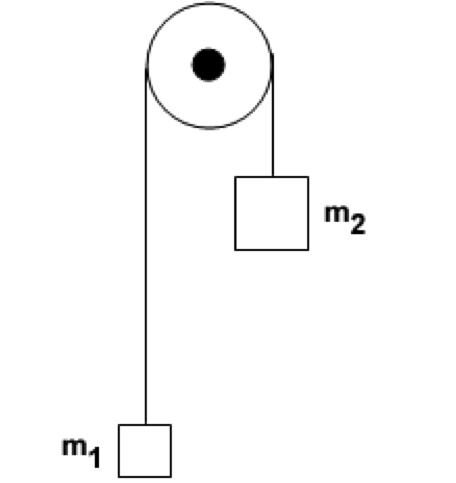
\includegraphics[scale=.8]{/Users/jgates/desktop/latex/pics/Atwood3}
\end{floatingfigure}
 
{\bf \Large{\arabic{ProbNum}}} An Atwood machine is constructed from a 3 kg mass and a 1 kg mass.  The 3 kg mass is released from rest 180 cm off of the floor, while the 1 kg mass is 40 cm above the floor.

\bigskip
Determine the speed of the 3 kg mass as it hits the floor.
\paragraph{}
\noindent
\vfill

After the 3 kg mass hits the floor, the 1 kg mass will continue to move upwards for a short time.  Determine how high above the floor the 1 kg mass will rise.
\vfill

Draw quantitatively correct acceleration and velocity graphs for the 1 kg mass.
\vfill
%\hfill 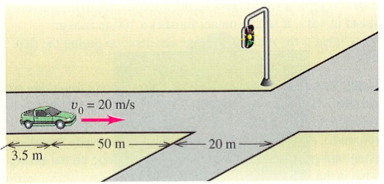
\includegraphics[scale=.85]{/Users/jgates/desktop/latex/pics/redlight.png}
\newpage